\subsection{Runtime Adaptation}
\label{sec:runtime}

\begin{figure}
  \centering
  \resizebox{\columnwidth}{!}{
    \begin{tikzpicture}
  %
  % Define basic styles
  %
  % Node
  \tikzstyle{module} = [draw, very thick, rounded corners,
  fill=white, minimum height=2.5em, inner sep=0.5em,
  rectangle, font={\bfseries}, align=center]
  \tikzstyle{cmodule} = [module, fill=black!20]

  % Edge
  \tikzstyle{stateEdgePortion} = [black, thick];
  \tikzstyle{dataEdge} = [stateEdgePortion, ->];
  \tikzstyle{controlEdgePartial} = [stateEdgePortion, dashed];
  \tikzstyle{controlEdge} = [controlEdgePartial, ->];
  \tikzstyle{controlDoubleEdge} = [controlEdgePartial, <->];
  \tikzstyle{edgeLabel} = [pos=0.5, text centered, font={\itshape}];

  \node[name=client, draw, very thick, fill=white,
  double copy shadow={shadow xshift=2pt, shadow yshift=-2pt, fill=white, draw},
  text height=13em, text width=31.5em] {};

  \node[name=server, draw, very thick, fill=white, draw,
  right=of client.north east, anchor=north west, xshift=1em,
  text height=7em, text width=12.5em] {};

  \node[module, name=source, below right=of client.north west,
  xshift=-1.5em, yshift=1.5em] {Source};
  \node[module, name=transform, right of=source, xshift=3.5em] {Transform};
  \node[cmodule, name=degrade, right of=transform, xshift=3.7em] {Degrade};
  \node[cmodule, name=queue, right of=degrade, xshift=3em] {Queue};
  \node[cmodule, name=socket, right of=queue, xshift=3em, text width=3em] {Socket};
  \node[cmodule, name=receiver, right of=socket, xshift=7em] {Receiver};
  \node[module, name=analytics, right of=receiver, xshift=3em] {Analytics};

  \node[cmodule, name=cc, at=($(queue)!0.5!(socket)$), yshift=-6em]
  {Congestion\\Controller};

  \draw ($(source.east)$) edge[dataEdge] ($(transform.west)$);
  \draw ($(transform.east)$) edge[dataEdge] ($(degrade.west)$);
  \draw ($(degrade.east)$) edge[dataEdge] ($(queue.west)$);
  \draw ($(queue.east)$) edge[dataEdge] ($(socket.west)$);
  \draw ($(socket.east)$) edge[dataEdge] node[edgeLabel, yshift=0.6em] {data}
  ($(receiver.west)$);
  \draw ($(receiver.east)$) edge[dataEdge] ($(analytics.west)$);

  %% Control path
  \draw let
  \p1 = ($(cc.center)$), \p2 = ($(degrade.center)$)
  in ($(cc.west)$) edge[controlEdgePartial] (\x2, \y1)
  (\x2, \y1) edge[controlEdge] ($(degrade.south)$);

  \draw let
  \p1 = ($(queue.south)$), \p2 = ($(cc.north)$)
  in ($(\x1, \y1) + (1em,0)$) edge[controlEdge] ($(\x1, \y2) + (1em,0)$);

  \draw let
  \p1 = ($(socket.south)$), \p2 = ($(cc.north)$)
  in ($(\x1, \y1) + (-1em,0)$) edge[controlDoubleEdge] ($(\x1, \y2) + (-1em,0)$);

  \node[name=clientlabel, above right=of client.south west, xshift=-2em, yshift=-2em] {Edge (Client)};
  \node[name=clientlabel, above left=of server.south east, xshift=2em, yshift=-2em] {Server};

  %%
  %% Legend
  %%
  \node[name=datalegend, below=1.5em of server.south west, xshift=2em]
  {\small Data Plane};
  \draw ($(datalegend.west) + (-2em, 0)$) edge[dataEdge]
  ($(datalegend.west) + (-0.5em, 0)$);

  \node[name=controllegend, below=2.5em of datalegend.west, anchor=west]
  {\small Control Plane};
  \draw ($(controllegend.west) + (-2em, 0)$) edge[controlEdge]
  ($(controllegend.west) + (-0.5em, 0)$);

  \node[name=applegend, right=3em of datalegend.east]
  {\small Application Logic};
  \node[module, name=applegendbox, left=0.1em of applegend, text width=0.3em,
  minimum height=0em] {};

  \node[name=syslegend, below=2.5em of applegend.west, anchor=west]
  {\small Runtime};
  \node[cmodule, name=syslegendbox, left=0.1em of syslegend, text width=0.3em,
  minimum size=0em] {};

\end{tikzpicture}

%%% Local Variables:
%%% mode: latex
%%% TeX-master: "sosp17"
%%% End:

  }
  % 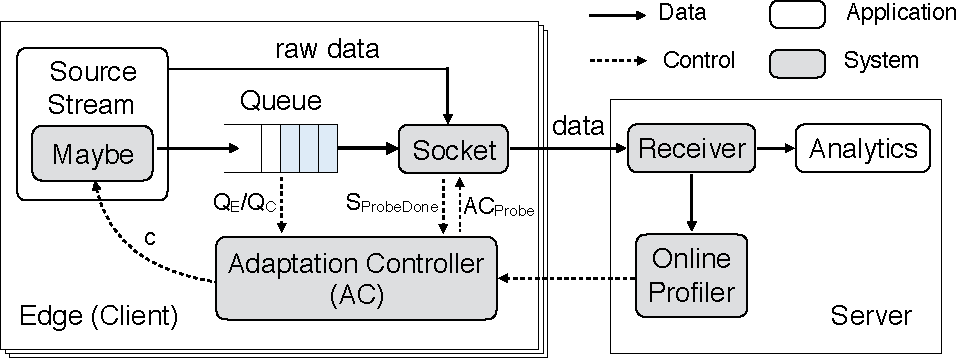
\includegraphics[width=\linewidth]{figures/runtime-adaptation.pdf}
  \caption{Runtime adaptation system architecture. The grey components are what
    \sysname{} provides.}
  \label{fig:runtime}
\end{figure}

At runtime, the user program is automatically converted to a client half and
server half; and \sysname{} abstracts the communication as well as rate
adaptation. \autoref{fig:runtime} shows our runtime architecture.

The data source with degradation is a module that supports \texttt{update}
function. To handle insufficient bandwidth, an object-level queue bridges data
generation (source) and the network IO. Followed by the queue is a socket module
that abstracts the network communication. It transmits data as fast as possible
and also supports traffic probing. The growth of the queue indicates congestions
and will trigger the congestion controller. The socket module estimates actual
available bandwidth. To avoid spikes in the bandwidth measurement, exponential
smoothing is employed.

At the core of our rate adjustment is a congestion control algorithms assisted
with stream data generation rate. We describe each state in details. Some of the
design is similar to BBR~\cite{cardwell2017bbr}.

\para{Startup behavior:} When the application starts up, it performs its first
(and most rapid) rate increase. On each \texttt{Q.NoQueue} received, it
decreases the level of degradation, hence an increase of the data rate.

\para{Reacting to congestion:} When congestion is detected by an increase of the
queued item, TCP's send rate is used as an approximation of the bottleneck
bandwidth of the current connection. \sysname{} then adjusts the level of
degradation such that the expected data rate is below the estimated
bandwidth. To allow the queue draining, we adjust the measured bandwidth with a
factor ALPHA (often 0.8). After the queue is drained and there is no queued item
for a configurable period, it fires \texttt{Q.NoQueue} event to the congestion
controller, which then enters into the \texttt{Steady} state.

\para{Steady state:} The steady state is the ideal state that the streaming
application should stay in. If currently the application is operating at the
maximum rate, then there is no need to probe. However, we might be in steady
state with degradation, in this case, we need to probe to test if there is more
bandwidth. Enter probe state.

\para{Probe for available bandwidth:} In contrast to BBR that adjusts the pace
of transmission, our probe is to send dummy traffic. If the application is
configured to run online profiling, then the probe traffic is the raw data.

% \begin{figure}
%   \centering
%   \resizebox{\columnwidth}{!}{
%     \begin{tikzpicture}[
  state/.style = { draw, very thick, fill=white, rounded corners=1em,
    minimum height=3em, minimum width=7em, node distance=7em, font={\bfseries},
    align=center },
  edge portion/.style = { black, thick },
  transition/.style = { edge portion, -> },
  algorithm/.style = { draw, thin, fill=white },
  ]

  \node [state] (startup) {
    STARTUP };
  \node [state] (congestion) [right=of startup] {CONGESTION};
  \draw [transition] (startup) -- (congestion)
  node [midway, auto] {Q.Congestion};

  \node [state] (steady) [below=of congestion] {STEADY};

  \draw [transition] ($(congestion.south west)!0.4!(congestion.south east)$)
  to node[midway, sloped, below] {Q.NoQueue}
  ($(steady.north west)!0.4!(steady.north east)$);

  \draw [transition] ($(steady.north west)!0.6!(steady.north east)$)
  to node[midway, sloped, below] {Q.Congestion}
  ($(congestion.south west)!0.6!(congestion.south east)$);

  \node [state] (probe) [left=of steady] {PROBE};

  \draw [transition] ($(steady.south west)!0.6!(steady.north west)$)
  -- ($(probe.south east)!0.6!(probe.north east)$)
  node[midway, auto, swap] {Q.Probe};

  \draw [transition, <-] ($(steady.south west)!0.4!(steady.north west)$)
  -- ($(probe.south east)!0.4!(probe.north east)$)
  node[midway, auto, align=left] {Q.Congestion | \\ IO.ProbeDone};

\end{tikzpicture}


%%% Local Variables:
%%% mode: latex
%%% TeX-master: "sosp17"
%%% End:

%   }
%   \caption{Congestion Control Algorithm}
%   \label{fig:cc}
% \end{figure}

\begin{figure}
  \centering
  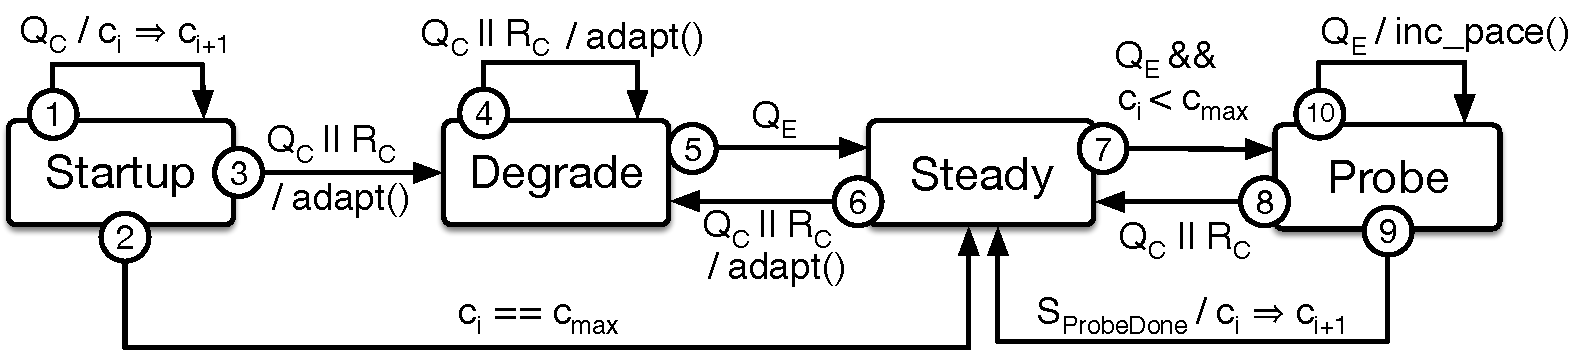
\includegraphics[width=\columnwidth]{figures/cc.pdf}
  \caption{Congestion Control Algorithm}
  \label{fig:cc}
\end{figure}

%%% Local Variables:
%%% mode: latex
%%% TeX-master: "sosp17"
%%% End:
